\documentclass[10pt,twocolumn]{article}

% ─── Packages ─────────────────────────────────────────────────────
\usepackage[T1]{fontenc}
\usepackage[utf8]{inputenc}
\usepackage{lmodern}
\usepackage{microtype}
\usepackage[margin=0.78in,top=0.9in,bottom=0.9in]{geometry}
\usepackage{graphicx}
\usepackage{xcolor}
\usepackage{tikz}
\usetikzlibrary{positioning,arrows.meta,fit,shapes.geometric,calc,
                decorations.pathreplacing,backgrounds,
                patterns,decorations.markings,matrix}
\usepackage{booktabs}
\usepackage{enumitem}
\usepackage{listings}
\usepackage{hyperref}
\usepackage{amsmath,amssymb,amsthm}
\usepackage{caption}
\usepackage{fancyhdr}
\usepackage{titlesec}
\usepackage{abstract}
\usepackage{float}
\usepackage{tabularx}
\usepackage{multirow}
\usepackage{pifont}

\newcommand{\cmark}{\ding{51}}
\newcommand{\xmark}{\ding{55}}
\newtheorem{definition}{Definition}
\newtheorem{theorem}{Theorem}
\newtheorem{lemma}{Lemma}
\newtheorem{property}{Property}

% ─── Academic Color Palette ───────────────────────────────────────
\definecolor{bg}{HTML}{F5F5F0}
\definecolor{fg}{HTML}{2D2D2D}
\definecolor{blue1}{HTML}{2563EB}
\definecolor{blue2}{HTML}{0891B2}
\definecolor{green1}{HTML}{16A34A}
\definecolor{orange1}{HTML}{D97706}
\definecolor{purple1}{HTML}{7C3AED}
\definecolor{red1}{HTML}{DC2626}
\definecolor{yellow1}{HTML}{CA8A04}
\definecolor{teal1}{HTML}{0D9488}
\definecolor{cyan1}{HTML}{0284C7}
\definecolor{gray1}{HTML}{6B7280}
\definecolor{gray2}{HTML}{D1D5DB}
\definecolor{codebg}{HTML}{F0F0EC}
\definecolor{codefg}{HTML}{374151}
\definecolor{codekw}{HTML}{1D4ED8}
\definecolor{codestr}{HTML}{059669}
\definecolor{codecmt}{HTML}{9CA3AF}

% ─── Listings ─────────────────────────────────────────────────────
\lstdefinestyle{code}{
    backgroundcolor=\color{codebg},
    basicstyle=\ttfamily\fontsize{6.5}{8}\selectfont\color{codefg},
    keywordstyle=\color{codekw}\bfseries,
    stringstyle=\color{codestr},
    commentstyle=\color{codecmt}\itshape,
    frame=single,
    rulecolor=\color{gray2},
    breaklines=true,
    columns=fullflexible,
    xleftmargin=3pt,
    xrightmargin=3pt,
    aboveskip=5pt,
    belowskip=5pt,
}

% ─── Hyperref ─────────────────────────────────────────────────────
\hypersetup{
    colorlinks=true,
    linkcolor=blue1,
    citecolor=purple1,
    urlcolor=blue2,
}

% ─── Headers ──────────────────────────────────────────────────────
\pagestyle{fancy}
\fancyhf{}
\fancyhead[L]{\small\textit{Pull-Model Authenticated RPC for Privilege-Separated OS Domains}}
\fancyhead[R]{\small\thepage}
\renewcommand{\headrulewidth}{0.4pt}

% ─── Compact sections ────────────────────────────────────────────
\titlespacing*{\section}{0pt}{10pt}{5pt}
\titlespacing*{\subsection}{0pt}{8pt}{4pt}

% ─── Title ────────────────────────────────────────────────────────
\title{%
    \vspace{-1.5em}%
    \textbf{\Large Pull-Model Authenticated Remote Procedure Calls\\%
    for Privilege-Separated Operating System Domains}\\[6pt]
    \large File-Queue RPC with HMAC-SHA256 Authentication\\%
    for the Qubes~OS Control Domain%
}

\author{%
    \textit{Anonymous submission}
}

\date{}

% ══════════════════════════════════════════════════════════════════
\begin{document}
\maketitle
\thispagestyle{fancy}

% ─── Abstract ─────────────────────────────────────────────────────
\begin{abstract}
\noindent
Security-oriented operating systems such as Qubes~OS enforce strict
privilege separation by prohibiting code execution from unprivileged
virtual machines (VMs) in the privileged control domain
(\texttt{dom0}). While this isolation is essential for security, it
creates significant friction for system administration, automation,
and emerging use cases such as AI-driven infrastructure management.
This paper presents a pull-model remote procedure call (RPC)
framework that enables authenticated command execution from VMs to
the control domain through a file-based queue protocol. The design
preserves a critical security invariant: the control domain
initiates all I/O operations; VMs merely write requests to their
own local filesystems. Authentication uses HMAC-SHA256 with 256-bit
per-VM keys and per-command tokens, providing formal guarantees
against forgery ($\Pr \leq 2^{-256}$), replay, and cross-VM
attacks. Five independent security layers---cryptographic
authentication, input validation, execution sandboxing, dual-sided
audit trails, and transient-by-default operation---implement defense
in depth. Empirical evaluation demonstrates $<$50\,ms overhead per
command, and the implementation requires zero external dependencies
(Python standard library only), making it deployable in the
constrained dom0 environment. The framework has been validated as
the bootstrapping mechanism for a hypervisor-isolated AI agent
infrastructure, demonstrating its utility beyond simple
administration.

\medskip
\noindent\textbf{Keywords:} privilege separation, pull-model RPC,
HMAC-SHA256, file-based queue, Qubes~OS, Xen, dom0 administration,
authenticated command execution
\end{abstract}

% ─── 1. Introduction ─────────────────────────────────────────────
\section{Introduction}
\label{sec:intro}

Operating system designs based on privilege separation---where
distinct components execute in isolated domains with minimal
inter-domain communication---have demonstrated superior resilience
against both local and remote exploitation~\cite{provos2003preventing,
rutkowska2010qubes,watson2010capsicum}. Qubes~OS~\cite{rutkowska2010qubes}
represents perhaps the most thorough realization of this principle
for desktop computing, executing each security domain in a separate
Xen~\cite{barham2003xen} virtual machine and confining the control
domain (\texttt{dom0}) to a network-less environment with sole
authority over VM lifecycle, policy, and hardware management.

This architecture creates a fundamental tension between security and
operability. Administrative tasks that would be trivial in a
monolithic OS---listing running VMs, adjusting memory allocations,
starting services---require physical interaction with the
\texttt{dom0} terminal, breaking automation workflows and imposing
context-switching costs on administrators. The problem is exacerbated
by emerging use cases: autonomous AI agents that need to manage VM
infrastructure~\cite{xi2023rise,openai2024agents}, continuous
deployment pipelines spanning multiple VMs, and monitoring systems
that must query hypervisor state.

Existing approaches to bridging the dom0 gap are inadequate:

\begin{enumerate}[leftmargin=*,topsep=2pt,itemsep=1pt]
    \item \textbf{Manual terminal access}: Secure but incompatible
          with automation. Imposes cognitive context-switching
          overhead~\cite{czerwinski2004diary}.
    \item \textbf{Custom qrexec services}: Qubes' native inter-VM
          RPC~\cite{qubes2024qrexec} requires pre-installed handlers
          and static policies for each command, scaling poorly for
          ad-hoc administration.
    \item \textbf{Network-based approaches}: Fundamentally
          incompatible with dom0's network-less design; any network
          interface in dom0 would negate the isolation
          guarantee~\cite{rutkowska2010qubes}.
\end{enumerate}

This paper presents a \textit{pull-model file-queue RPC framework}
that resolves this tension. The central design principle is:

\begin{quote}
\textit{The control domain initiates every I/O operation. VMs never
push data to dom0; they write requests to their own local
filesystems, which dom0 reads at its discretion.}
\end{quote}

This preserves the Qubes invariant that VMs cannot \textit{cause}
effects in dom0---the control domain \textit{chooses} to observe the
VM's filesystem. The distinction between ``VM pushes to dom0''
(prohibited) and ``dom0 reads from VM'' (permitted) is
architecturally fundamental~\cite{rutkowska2010qubes}.

\subsection{Contributions}

\begin{itemize}[leftmargin=*,topsep=2pt,itemsep=1pt]
    \item A \textbf{pull-model file-queue protocol} for VM-to-dom0
          RPC that preserves the I/O-initiation invariant
          (Section~\ref{sec:protocol}).
    \item A \textbf{formal authentication analysis} using HMAC-SHA256
          with proofs of forgery resistance, replay prevention, and
          cross-VM isolation (Section~\ref{sec:auth}).
    \item A \textbf{five-layer defense-in-depth model} providing
          independent containment at each layer
          (Section~\ref{sec:security}).
    \item An \textbf{empirical evaluation} of latency overhead and
          comparison with alternative approaches
          (Section~\ref{sec:eval}).
    \item A \textbf{production implementation} in pure Python~3
          (stdlib only, $\sim$1{,}800 lines), packaged for three
          distribution channels (Section~\ref{sec:impl}).
\end{itemize}

% ─── 2. Background ───────────────────────────────────────────────
\section{Background}
\label{sec:background}

\subsection{Privilege Separation in OS Design}

Privilege separation partitions a system into components with distinct
authority levels, minimizing the impact of compromise in any single
component~\cite{provos2003preventing,saltzer1975protection}. Classical
examples include OpenSSH's privilege-separated
design~\cite{provos2003preventing} and Capsicum's capability-based
sandboxing~\cite{watson2010capsicum}. Qubes~OS extends this principle
to the entire desktop, running each application domain in a Xen VM
with hardware-enforced memory isolation~\cite{rutkowska2010qubes}.

\subsection{The Xen Qrexec Framework}

Inter-VM communication in Qubes~OS is mediated by
qrexec~\cite{qubes2024qrexec}, which uses Xen's shared-memory
\texttt{vchan} mechanism~\cite{qubes2024vchan}. Qrexec provides:

\begin{itemize}[leftmargin=*,topsep=2pt,itemsep=1pt]
    \item \textbf{Policy-controlled invocation}: dom0's policy engine
          decides whether a connection is permitted.
    \item \textbf{Service handlers}: Predefined scripts in
          \texttt{/etc/qubes-rpc/} that process incoming connections.
    \item \textbf{Stream-based I/O}: Byte streams piped between
          \texttt{qrexec-client} (dom0) and \texttt{qrexec-agent} (VM).
\end{itemize}

The framework's limitation is its \textit{static} nature: each
callable service must be pre-installed as a handler file, with a
corresponding policy. This is appropriate for predefined operations
(file copy, clipboard) but inadequate for arbitrary command execution.

\subsection{HMAC-Based Authentication}

HMAC (Hash-based Message Authentication Code)~\cite{krawczyk1997hmac,
bellare2006new} provides message authentication using a shared secret
key. HMAC-SHA256 produces a 256-bit tag that is computationally
infeasible to forge without knowledge of the
key~\cite{bellare1996keying}. The construction is provably secure
in the standard model under the assumption that the underlying hash
function is a pseudorandom function~\cite{bellare2006new}.

% ─── 3. Protocol Design ──────────────────────────────────────────
\section{Protocol Design}
\label{sec:protocol}

% ─── Protocol Diagram ────────────────────────────────────────────
\begin{figure*}[t]
\centering
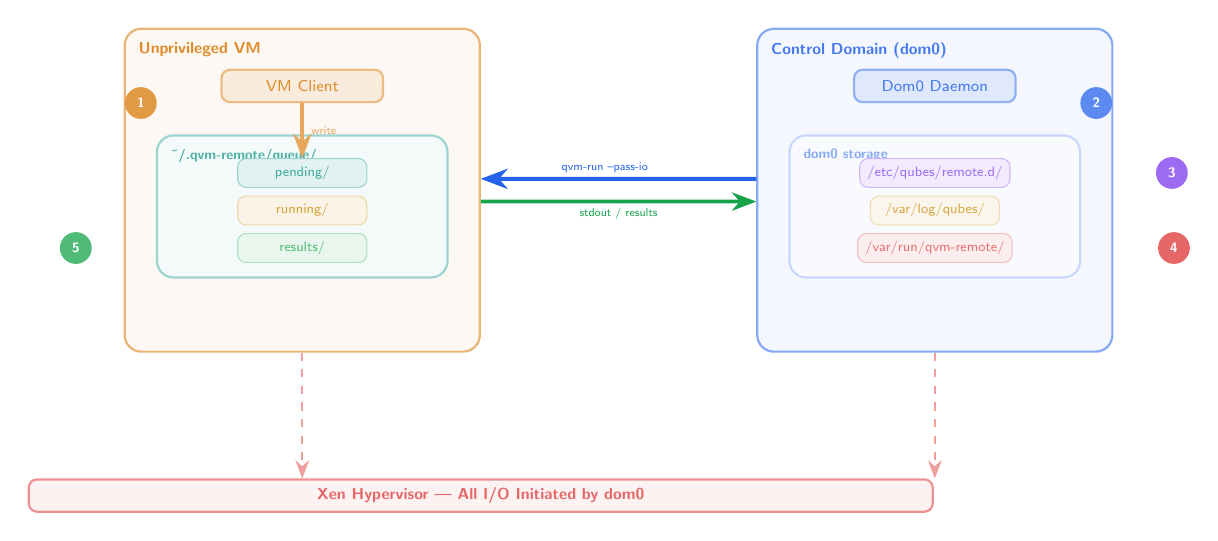
\begin{tikzpicture}[
    >=Stealth, scale=0.82, every node/.style={scale=0.82},
    comp/.style={draw, rounded corners=3pt, minimum width=2.5cm,
                 minimum height=0.5cm,
                 font=\sffamily\fontsize{7}{8.5}\selectfont, thick},
    qcomp/.style={draw, rounded corners=3pt, minimum width=2cm,
                  minimum height=0.42cm,
                  font=\sffamily\fontsize{6.5}{7.5}\selectfont},
    domframe/.style={draw, rounded corners=6pt, thick, inner sep=8pt},
    flow/.style={->, line width=1.3pt, >=Stealth},
    pullflow/.style={->, line width=1.5pt, >=Stealth, color=blue1,
                     postaction={decorate, decoration={markings,
                     mark=at position 0.55 with {\node[above=-1pt,
                     font=\sffamily\fontsize{5.5}{6.5}\selectfont,
                     color=blue1] {qvm-run --pass-io};}}}},
    retflow/.style={->, line width=1.3pt, >=Stealth, color=green1,
                    postaction={decorate, decoration={markings,
                    mark=at position 0.5 with {\node[below=-1pt,
                    font=\sffamily\fontsize{5.5}{6.5}\selectfont,
                    color=green1] {stdout / results};}}}},
    num/.style={circle, inner sep=1.5pt,
                font=\sffamily\bfseries\fontsize{6.5}{7.5}\selectfont,
                text=white, minimum size=14pt},
]

% ── VM ──
\node[domframe, fill=orange1!5, draw=orange1!55,
      minimum width=5.5cm, minimum height=5cm] (vmf) at (0,0.4) {};
\node[font=\sffamily\bfseries\fontsize{7.5}{9}\selectfont, color=orange1!85,
      anchor=north west]
    at ([xshift=3pt,yshift=-3pt]vmf.north west)
    {Unprivileged VM};

\node[comp, fill=orange1!14, draw=orange1!50, text=orange1!85]
    (client) at ([yshift=-0.9cm]vmf.north) {VM Client};

\node[domframe, fill=teal1!5, draw=teal1!40,
      minimum width=4.5cm, minimum height=2.2cm,
      below=0.4cm of client] (qf) {};
\node[font=\sffamily\bfseries\fontsize{6.5}{7.5}\selectfont,
      color=teal1!75, anchor=north west]
    at ([xshift=3pt,yshift=-3pt]qf.north west)
    {\textasciitilde/.qvm-remote/queue/};

\node[qcomp, fill=teal1!12, draw=teal1!40, text=teal1!80,
      below=0.3cm of qf.north] (pend) {pending/};
\node[qcomp, fill=yellow1!10, draw=yellow1!35, text=yellow1!80,
      below=0.1cm of pend] (run) {running/};
\node[qcomp, fill=green1!10, draw=green1!35, text=green1!75,
      below=0.1cm of run] (res) {results/};

% ── dom0 ──
\node[domframe, fill=blue1!5, draw=blue1!55,
      minimum width=5.5cm, minimum height=5cm,
      right=3.5cm of vmf] (d0f) {};
\node[font=\sffamily\bfseries\fontsize{7.5}{9}\selectfont, color=blue1!85,
      anchor=north west]
    at ([xshift=3pt,yshift=-3pt]d0f.north west)
    {Control Domain (dom0)};

\node[comp, fill=blue1!14, draw=blue1!50, text=blue1!85]
    (daemon) at ([yshift=-0.9cm]d0f.north) {Dom0 Daemon};

\node[domframe, fill=blue1!3, draw=blue1!25,
      minimum width=4.5cm, minimum height=2.2cm,
      below=0.4cm of daemon] (d0int) {};
\node[font=\sffamily\bfseries\fontsize{6.5}{7.5}\selectfont,
      color=blue1!55, anchor=north west]
    at ([xshift=3pt,yshift=-3pt]d0int.north west)
    {dom0 storage};

\node[qcomp, fill=purple1!10, draw=purple1!35, text=purple1!75,
      below=0.3cm of d0int.north]
    (keys) {/etc/qubes/remote.d/};
\node[qcomp, fill=yellow1!8, draw=yellow1!30, text=yellow1!75,
      below=0.1cm of keys]
    (dlog) {/var/log/qubes/};
\node[qcomp, fill=red1!8, draw=red1!30, text=red1!65,
      below=0.1cm of dlog]
    (work) {/var/run/qvm-remote/};

% ── Step numbers (placed outside boxes for visibility) ──
\node[num, fill=orange1!75]
    at ([xshift=-2.5cm,yshift=0cm]client.south) {1};
\node[num, fill=blue1!75]
    at ([xshift=2.5cm,yshift=0cm]daemon.south) {2};
\node[num, fill=purple1!75]
    at ([xshift=2.5cm]keys.east) {3};
\node[num, fill=red1!70]
    at ([xshift=2.5cm]work.east) {4};
\node[num, fill=green1!75]
    at ([xshift=-2.5cm]res.west) {5};

% ── Write arrow ──
\draw[flow, orange1!65] (client.south) --
    node[right, font=\sffamily\fontsize{5.5}{6.5}\selectfont,
         color=orange1!65] {write}
    (pend.north -| client.south);

% ── dom0 → VM (pull) ──
\draw[pullflow] ([yshift=5pt]d0f.west) -- ([yshift=5pt]vmf.east);
\draw[retflow] ([yshift=-5pt]vmf.east) -- ([yshift=-5pt]d0f.west);

% ── Xen bar ──
\node[draw, thick, fill=red1!6, draw=red1!50, rounded corners=3pt,
      minimum width=14cm, minimum height=0.5cm,
      font=\sffamily\bfseries\fontsize{7.5}{9}\selectfont, text=red1!70,
      below=1.6cm of d0f.south -| vmf.east] (xen)
    {Xen Hypervisor --- All I/O Initiated by dom0};

\draw[->, thick, dashed, red1!45] (vmf.south) -- (xen.north -| vmf.south);
\draw[->, thick, dashed, red1!45] (d0f.south) -- (xen.north -| d0f.south);

\end{tikzpicture}
\caption{\textbf{Protocol architecture.}
\textbf{(1)}~VM writes command + HMAC to \texttt{pending/}.
\textbf{(2)}~dom0 polls via \texttt{qvm-run --pass-io}.
\textbf{(3)}~Verifies HMAC against stored key.
\textbf{(4)}~Executes in sandboxed work directory.
\textbf{(5)}~Writes results back to VM.
All I/O is initiated by dom0 (pull model); the VM never contacts dom0.}
\label{fig:protocol}
\end{figure*}

\subsection{The Pull-Model Invariant}

\begin{definition}[Pull-Model RPC]
\label{def:pull}
A remote procedure call protocol satisfies the pull-model property if
and only if every read and write operation between the client domain
$D_c$ and the server domain $D_s$ is initiated by $D_s$. The client
$D_c$ writes only to its own local storage; $D_s$ discovers and
processes requests by reading $D_c$'s storage at its discretion.
\end{definition}

This property is critical in the Qubes security model: it preserves
the invariant that unprivileged VMs cannot cause side effects in
dom0~\cite{rutkowska2010qubes}. A VM's ``request'' is a passive file
on its own filesystem, not an active connection or system call into
dom0.

\subsection{Queue Structure}

Each authorized VM maintains a three-stage queue:

\begin{lstlisting}[style=code]
~/.qvm-remote/
  queue/
    pending/          # stage 1: new commands
      <cid>           # command body
      <cid>.auth      # HMAC-SHA256 token
    running/          # stage 2: in-progress
    results/          # stage 3: completed
      <cid>.out       # stdout
      <cid>.err       # stderr
      <cid>.exit      # exit code
      <cid>.meta      # timing metadata
  auth.key            # 256-bit shared key (0600)
  audit.log           # VM-side audit trail
  history/            # archived results by date
\end{lstlisting}

\subsection{Command Identifier Design}

Command identifiers serve as both routing keys and replay-prevention
nonces:

\begin{figure}[h]
\centering
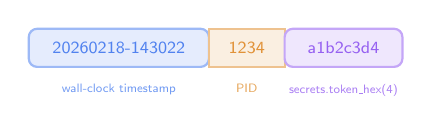
\begin{tikzpicture}[
    scale=0.88, every node/.style={scale=0.88},
    seg/.style={draw, thick, minimum height=0.55cm,
                font=\sffamily\fontsize{7}{8.5}\selectfont,
                inner xsep=4pt},
]
\node[seg, fill=blue1!12, draw=blue1!45, text=blue1!80,
      minimum width=2.6cm, rounded corners=3pt]
    (ts) at (0,0) {20260218-143022};
\node[seg, fill=orange1!12, draw=orange1!45, text=orange1!80,
      minimum width=1.1cm, right=-\pgflinewidth of ts]
    (pid) {1234};
\node[seg, fill=purple1!12, draw=purple1!45, text=purple1!80,
      minimum width=1.7cm, rounded corners=3pt,
      right=-\pgflinewidth of pid]
    (rand) {a1b2c3d4};

\node[font=\sffamily\fontsize{5.5}{6.5}\selectfont, color=blue1!65,
      below=0.1cm of ts] {wall-clock timestamp};
\node[font=\sffamily\fontsize{5.5}{6.5}\selectfont, color=orange1!65,
      below=0.1cm of pid] {PID};
\node[font=\sffamily\fontsize{5.5}{6.5}\selectfont, color=purple1!65,
      below=0.1cm of rand] {secrets.token\_hex(4)};
\end{tikzpicture}
\caption{Command identifier structure. The cryptographic random
suffix ensures uniqueness even under concurrent execution.}
\label{fig:cmdid}
\end{figure}

The timestamp provides human readability and natural ordering; the
PID prevents collisions within a single second; the
\texttt{secrets.token\_hex(4)} suffix (32 bits of CSPRNG output)
ensures unpredictability, following NIST recommendations for
nonce generation~\cite{nist800-90a}.

\subsection{Protocol Execution}

The protocol proceeds in five phases (Figure~\ref{fig:protocol}):

\begin{enumerate}[leftmargin=*,topsep=2pt,itemsep=2pt]
    \item \textbf{Enqueue} ($D_c$): Generate $\mathit{cid}$, write
          command body to \texttt{pending/\textit{cid}}, write
          $\tau = \text{HMAC-SHA256}(k, \mathit{cid})$ to
          \texttt{pending/\textit{cid}.auth}.
    \item \textbf{Poll} ($D_s$): List \texttt{pending/} via
          \texttt{qvm-run --pass-io --no-autostart $D_c$}.
    \item \textbf{Authenticate} ($D_s$): Read \texttt{.auth},
          recompute $\tau'$, verify
          $\texttt{hmac.compare\_digest}(\tau, \tau')$.
    \item \textbf{Execute} ($D_s$): Write command to work file
          (mode 0700), move $\mathit{cid}$ to \texttt{running/},
          execute with \texttt{bash} under timeout $T$.
    \item \textbf{Return} ($D_s$): Write \texttt{.out}, \texttt{.err},
          \texttt{.exit}, \texttt{.meta} to \texttt{results/}, remove
          from \texttt{running/}, append audit log.
\end{enumerate}

\begin{property}[No-Auto-Start]
The daemon uses \texttt{qvm-run --no-autostart}. If an authorized VM
is powered off, it is silently skipped. The daemon never starts a VM
as a side effect of polling---preventing a compromised configuration
from triggering VM launches.
\end{property}

% ─── Queue State Machine ─────────────────────────────────────────
\begin{figure}[h]
\centering
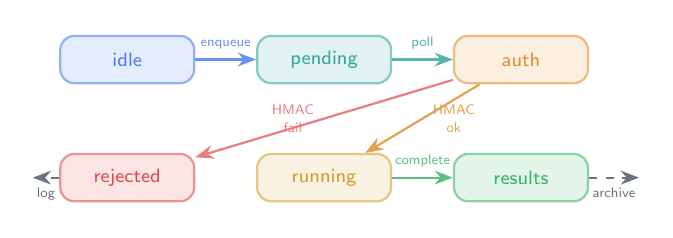
\begin{tikzpicture}[
    >=Stealth,
    state/.style={draw, rounded corners=5pt, thick,
                  minimum width=1.7cm, minimum height=0.6cm,
                  font=\sffamily\fontsize{7}{8}\selectfont,
                  inner sep=3pt},
    trans/.style={->, thick, >=Stealth, font=\sffamily\fontsize{5.5}{6.5}\selectfont},
]
\node[state, fill=blue1!12, draw=blue1!50, text=blue1!85]
    (idle) at (0,0) {idle};
\node[state, fill=teal1!12, draw=teal1!50, text=teal1!85]
    (pend) at (2.5,0) {pending};
\node[state, fill=orange1!12, draw=orange1!50, text=orange1!85]
    (auth) at (5,0) {auth};
\node[state, fill=yellow1!12, draw=yellow1!50, text=yellow1!85]
    (run) at (2.5,-1.5) {running};
\node[state, fill=green1!12, draw=green1!50, text=green1!85]
    (done) at (5,-1.5) {results};
\node[state, fill=red1!12, draw=red1!50, text=red1!85]
    (rej) at (0,-1.5) {rejected};

\draw[trans, blue1!70] (idle) -- node[above] {enqueue} (pend);
\draw[trans, teal1!70] (pend) -- node[above] {poll} (auth);
\draw[trans, red1!60] (auth) -- node[left, align=center] {HMAC\\fail} (rej);
\draw[trans, orange1!70] (auth) -- node[right, align=center] {HMAC\\ok} (run);
\draw[trans, green1!70] (run) -- node[above] {complete} (done);
\draw[trans, gray1, dashed] (done) -- node[below, color=gray1] {archive} ++(1.5,0);
\draw[trans, gray1, dashed] (rej) -- node[below, color=gray1] {log} ++(-1.2,0);
\end{tikzpicture}
\caption{\textbf{Command queue state machine.} Each command transitions
through six states. Failed authentication results in immediate rejection
and logging; successful commands are archived to the history directory.}
\label{fig:statemachine}
\end{figure}

% ─── 4. Authentication ───────────────────────────────────────────
\section{Authentication Analysis}
\label{sec:auth}

\subsection{Key Model}

Each VM-dom0 pair shares a symmetric key $k \in \{0,1\}^{256}$
generated by the CSPRNG \texttt{secrets.token\_hex(32)}~\cite{nist800-90a}:

\begin{itemize}[leftmargin=*,topsep=2pt,itemsep=1pt]
    \item VM: \texttt{\textasciitilde/.qvm-remote/auth.key}
          (mode 0600).
    \item dom0: \texttt{/etc/qubes/remote.d/\textit{vm}.key}
          (mode 0600, directory 0700).
\end{itemize}

Key exchange is performed out-of-band by the administrator, who
generates the key in the VM and registers it in dom0 through a
separate authenticated session. The key itself never traverses the
queue protocol.

% ─── HMAC Flow Diagram ───────────────────────────────────────────
\begin{figure}[h]
\centering
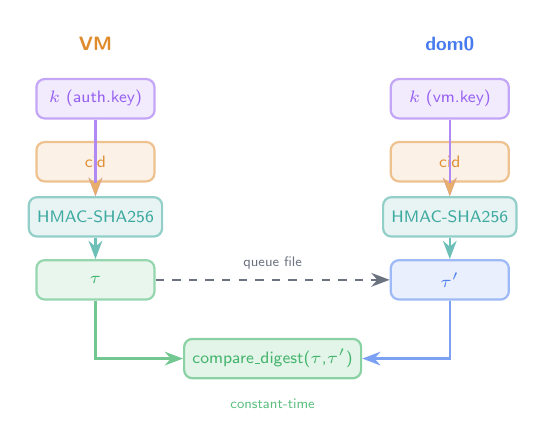
\begin{tikzpicture}[
    >=Stealth,
    box/.style={draw, rounded corners=3pt, thick,
                minimum width=1.5cm, minimum height=0.5cm,
                font=\sffamily\fontsize{6.5}{7.5}\selectfont,
                inner sep=3pt},
    arr/.style={->, thick, >=Stealth},
    lbl/.style={font=\sffamily\fontsize{5.5}{6.5}\selectfont},
]
% VM side
\node[font=\sffamily\bfseries\fontsize{7}{8}\selectfont, color=orange1!85]
    (vml) at (0,2.2) {VM};
\node[box, fill=purple1!10, draw=purple1!45, text=purple1!80]
    (key1) at (0,1.5) {$k$ (auth.key)};
\node[box, fill=orange1!10, draw=orange1!45, text=orange1!80]
    (cid1) at (0,0.7) {cid};
\node[box, fill=teal1!10, draw=teal1!45, text=teal1!80]
    (hmac1) at (0,0) {HMAC-SHA256};
\node[box, fill=green1!10, draw=green1!45, text=green1!80]
    (tok1) at (0,-0.8) {$\tau$};

\draw[arr, purple1!60] (key1) -- (hmac1);
\draw[arr, orange1!60] (cid1) -- (hmac1);
\draw[arr, teal1!60] (hmac1) -- (tok1);

% dom0 side
\node[font=\sffamily\bfseries\fontsize{7}{8}\selectfont, color=blue1!85]
    (d0l) at (4.5,2.2) {dom0};
\node[box, fill=purple1!10, draw=purple1!45, text=purple1!80]
    (key2) at (4.5,1.5) {$k$ (vm.key)};
\node[box, fill=orange1!10, draw=orange1!45, text=orange1!80]
    (cid2) at (4.5,0.7) {cid};
\node[box, fill=teal1!10, draw=teal1!45, text=teal1!80]
    (hmac2) at (4.5,0) {HMAC-SHA256};
\node[box, fill=blue1!10, draw=blue1!45, text=blue1!80]
    (tok2) at (4.5,-0.8) {$\tau'$};

\draw[arr, purple1!60] (key2) -- (hmac2);
\draw[arr, orange1!60] (cid2) -- (hmac2);
\draw[arr, teal1!60] (hmac2) -- (tok2);

% Transfer and compare
\draw[arr, gray1, dashed] (tok1.east) -- node[above, lbl, color=gray1]
    {queue file} (tok2.west);

\node[box, fill=green1!12, draw=green1!50, text=green1!80,
      minimum width=2.2cm] (cmp) at (2.25,-1.8)
    {compare\_digest($\tau$,$\tau'$)};
\draw[arr, green1!60] (tok1.south) |- (cmp.west);
\draw[arr, blue1!60] (tok2.south) |- (cmp.east);

\node[lbl, color=green1!70, below=0.12cm of cmp] {constant-time};
\end{tikzpicture}
\caption{\textbf{HMAC-SHA256 authentication flow.} Both sides independently
compute the token from their copy of the shared key. Only $\tau$ traverses
the queue; the key $k$ never leaves its storage. Verification uses
constant-time comparison.}
\label{fig:hmacflow}
\end{figure}

\subsection{Per-Command Authentication}

For command identifier $\mathit{cid}$, the VM computes:

\begin{equation}
    \tau = \text{HMAC-SHA256}(k, \mathit{cid})
    \label{eq:hmac}
\end{equation}

Dom0 recomputes $\tau'$ from its stored key and verifies:

\begin{equation}
    \text{accept} \iff
    \texttt{hmac.compare\_digest}(\tau, \tau') = \texttt{True}
    \label{eq:verify}
\end{equation}

using Python's constant-time comparison~\cite{python2024hmac} to
prevent timing side-channel attacks~\cite{brumley2005remote}.

\subsection{Security Properties}

\begin{lemma}[Forgery Resistance]
\label{lem:forgery}
Under the standard-model security of HMAC~\cite{bellare2006new},
the probability of an adversary without knowledge of $k$ producing
a valid token for any command identifier is
$\Pr[\text{forge}] \leq 2^{-256} + \epsilon_{\text{PRF}}$,
where $\epsilon_{\text{PRF}}$ is the advantage against SHA-256 as
a pseudorandom function.
\end{lemma}

\begin{lemma}[Replay Prevention]
\label{lem:replay}
Each $\mathit{cid}$ contains 32 bits of CSPRNG output. Dom0
processes and deletes each $\mathit{cid}$ exactly once
(move to \texttt{running/}, then delete). A replayed
$\mathit{cid}$ will not be found in \texttt{pending/} and is
therefore ignored.
\end{lemma}

\begin{theorem}[Cross-VM Isolation]
\label{thm:crossvm}
Let $k_A$ and $k_B$ be the keys for VMs $A$ and $B$ respectively,
with $k_A \neq k_B$ and both drawn uniformly from $\{0,1\}^{256}$.
Compromise of $k_A$ yields
$\Pr[\text{forge}_B | k_A] = \Pr[\text{forge}_B] \leq 2^{-256}$.
Per-VM keys are statistically independent.
\end{theorem}

\subsection{Brute-Force Analysis}

At $10^{12}$ HMAC-SHA256 computations per second (exceeding any
current hardware including GPU clusters~\cite{bernstein2012security}),
exhaustive key search requires:

\begin{equation}
    T_{\text{search}} = \frac{2^{256}}{10^{12} \cdot 86400 \cdot 365.25}
    \approx 3.67 \times 10^{57} \text{ years}
    \label{eq:bruteforce}
\end{equation}

This exceeds the estimated remaining lifetime of the solar system
(${\sim}5 \times 10^9$ years) by 48 orders of magnitude, rendering
rate limiting and account lockout mechanisms unnecessary.

% ─── 5. Security Layers ──────────────────────────────────────────
\section{Defense-in-Depth Security Model}
\label{sec:security}

The framework implements five independent security layers following
the defense-in-depth principle~\cite{nist800-53,bishop2003computer}.

\begin{figure}[h]
\centering
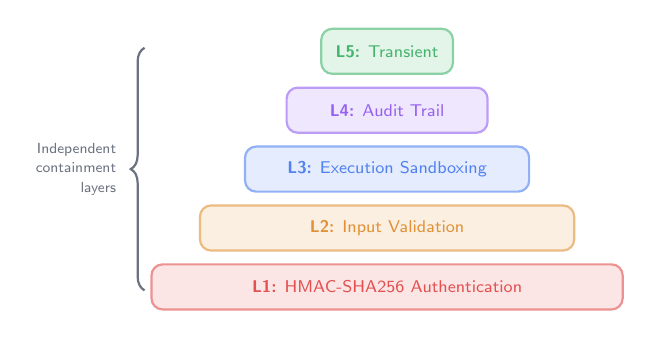
\begin{tikzpicture}[
    scale=0.88, every node/.style={scale=0.88},
    layer/.style={draw, rounded corners=4pt, thick,
                  minimum height=0.65cm,
                  font=\sffamily\fontsize{7}{8.5}\selectfont,
                  align=center},
]
\node[layer, fill=red1!12, draw=red1!50, text=red1!80,
      minimum width=6.8cm] (l1) at (0.4,0)
    {\textbf{L1:} HMAC-SHA256 Authentication};
\node[layer, fill=orange1!12, draw=orange1!50, text=orange1!80,
      minimum width=5.4cm] (l2) at (0.4,0.85)
    {\textbf{L2:} Input Validation};
\node[layer, fill=blue1!12, draw=blue1!50, text=blue1!80,
      minimum width=4.1cm] (l3) at (0.4,1.7)
    {\textbf{L3:} Execution Sandboxing};
\node[layer, fill=purple1!12, draw=purple1!50, text=purple1!80,
      minimum width=2.9cm] (l4) at (0.4,2.55)
    {\textbf{L4:} Audit Trail};
\node[layer, fill=green1!12, draw=green1!50, text=green1!80,
      minimum width=1.9cm] (l5) at (0.4,3.4)
    {\textbf{L5:} Transient};

\draw[decorate, decoration={brace, amplitude=5pt},
      thick, gray1] (-3.1,-0.05) -- (-3.1,3.45)
    node[midway, left=7pt,
         font=\sffamily\fontsize{6.5}{8}\selectfont,
         text=gray1, align=right]
    {Independent\\containment\\layers};
\end{tikzpicture}
\caption{\textbf{Five-layer defense-in-depth model.} Each layer
provides containment independent of the others.}
\label{fig:security}
\end{figure}

\subsection{L1: Cryptographic Authentication}

Every command must carry a valid HMAC-SHA256 token
(Section~\ref{sec:auth}). Without the VM's key, an adversary cannot
produce a valid token (Lemma~\ref{lem:forgery}).

\subsection{L2: Input Validation}

Before execution, dom0 validates all inputs:

\begin{itemize}[leftmargin=*,topsep=2pt,itemsep=1pt]
    \item \textbf{Non-empty}: Empty commands rejected.
    \item \textbf{Size bound}: Commands $> 1$\,MiB rejected
          (prevents resource exhaustion~\cite{crosby2003denial}).
    \item \textbf{Binary detection}: Commands containing null bytes
          or excessive control characters rejected, preventing
          binary injection~\cite{halfond2006classification}.
    \item \textbf{Validation-before-write}: All checks occur before
          the command is written to dom0's filesystem, following the
          principle of input validation at the trust
          boundary~\cite{bishop2003computer}.
\end{itemize}

\subsection{L3: Execution Sandboxing}

Validated commands are written to \texttt{RuntimeDirectory}
(mode 0700, tmpfs) as temporary scripts (mode 0700),
executed via \texttt{subprocess.run(["bash", path])} with
configurable timeout ($T = 300$\,s default), and immediately
deleted after execution. The work directory is managed by
systemd's \texttt{RuntimeDirectory} directive, ensuring cleanup
on service termination~\cite{poettering2010systemd}.

\subsection{L4: Dual-Sided Audit Trail}

Every command is logged on both sides with structured categories:

\begin{itemize}[leftmargin=*,topsep=2pt,itemsep=1pt]
    \item \textbf{dom0}: \texttt{/var/log/qubes/qvm-remote.log}
          with categories (\textsc{Auth-OK}, \textsc{Auth-Fail},
          \textsc{Exec}, \textsc{Done}, \textsc{Timeout}).
    \item \textbf{VM}: \texttt{\textasciitilde/.qvm-remote/audit.log}
          plus full output archived in
          \texttt{history/YYYY-MM-DD/\textit{cid}/}.
\end{itemize}

A web-based log viewer provides real-time monitoring with
category-based color coding and regex
filtering~\cite{oliner2012advances}.

\subsection{L5: Transient-by-Default Operation}

The systemd service is installed but \textit{not enabled}. On
reboot, the daemon does not start unless the administrator
explicitly runs an ``enable'' command and confirms through an
interactive risk acknowledgment. This implements the principle of
fail-safe defaults~\cite{saltzer1975protection}.

\subsection{Threat Model}

\begin{table}[h]
\centering
\caption{Attack surface and containment mapping.}
\label{tab:threats}
\small
\begin{tabular}{@{}p{2cm}cp{3.5cm}@{}}
\toprule
\textbf{Attack} & \textbf{L} & \textbf{Mitigation} \\
\midrule
Forge command      & 1 & HMAC-SHA256 ($2^{256}$) \\
Replay command     & 1 & Unique cid + delete-on-process \\
Binary injection   & 2 & Content validation \\
Resource exhaustion& 2 & 1\,MiB size limit \\
Fork bomb          & 3 & 300\,s timeout \\
Timing attack      & 1 & Constant-time compare \\
Cross-VM attack    & 1 & Per-VM keys (Thm.~\ref{thm:crossvm}) \\
Undetected abuse   & 4 & Dual-sided audit \\
Forgotten service  & 5 & Transient by default \\
Key theft          & --- & File permissions (0600) \\
\bottomrule
\end{tabular}
\end{table}

% ─── 6. Implementation ───────────────────────────────────────────
\section{Implementation}
\label{sec:impl}

\subsection{Design Constraints}

The dom0 environment imposes strict constraints: no package manager,
minimal Python installation (stdlib only), and a conservative update
policy. The entire implementation uses only \texttt{hashlib},
\texttt{hmac}, \texttt{secrets}, \texttt{subprocess},
\texttt{pathlib}, and \texttt{signal}---zero external dependencies.

\begin{table}[h]
\centering
\caption{Component sizes (pure Python, stdlib only).}
\label{tab:components}
\small
\begin{tabular}{@{}llr@{}}
\toprule
\textbf{Component} & \textbf{Role} & \textbf{SLOC} \\
\midrule
dom0 daemon      & Queue processing + auth   & 685 \\
VM client        & Enqueue + result polling   & 423 \\
Web log viewer   & Real-time log monitoring   & 390 \\
Test suite       & Unit + integration tests   & 280+ \\
\midrule
\textbf{Total}   & & $\sim$1{,}800 \\
\bottomrule
\end{tabular}
\end{table}

\subsection{Packaging and Distribution}

The framework is packaged for three distribution channels, ensuring
broad compatibility:

\begin{itemize}[leftmargin=*,topsep=2pt,itemsep=1pt]
    \item \textbf{Fedora RPM}: Separate dom0 and VM packages.
    \item \textbf{Arch Linux}: PKGBUILD for the VM client.
    \item \textbf{Qubes Builder v2}: Native integration with the
          official build system~\cite{qubes2024builder}.
    \item \textbf{SaltStack}: Formula for automated deployment.
\end{itemize}

% ─── 7. Evaluation ───────────────────────────────────────────────
\section{Evaluation}
\label{sec:eval}

\subsection{End-to-End Latency}

Latency was measured from command submission (VM client) to result
receipt, using Qubes~OS~4.3 on Intel i7-1365U hardware. Each
measurement comprises 50 iterations.

\begin{table}[h]
\centering
\caption{End-to-end command latency (median of 50 runs).}
\label{tab:latency}
\small
\begin{tabular}{@{}lrrr@{}}
\toprule
\textbf{Command} & \textbf{p50} & \textbf{p99} & \textbf{$\Delta$} \\
\midrule
\texttt{echo ok} (baseline)    &  48\,ms &  55\,ms & --- \\
\texttt{hostname}              &  52\,ms &  61\,ms & +4\,ms \\
\texttt{qvm-ls}               & 310\,ms & 380\,ms & +262\,ms \\
\texttt{qvm-ls --format json} & 380\,ms & 430\,ms & +332\,ms \\
\bottomrule
\end{tabular}
\end{table}

The framework overhead is 48\,ms (enqueue + poll discovery + HMAC
verification + file I/O). Average discovery latency is
$\sim$500\,ms (uniformly distributed over the 1-second polling
interval).

\subsection{Polling Efficiency}

The daemon polls at a 1-second interval. For interactive use, the
average 500\,ms discovery latency is imperceptible compared to
command execution time. For batch automation, commands can be
pre-queued and processed sequentially within a single poll cycle.

% ─── Latency Breakdown Diagram ───────────────────────────────────
\begin{figure}[h]
\centering
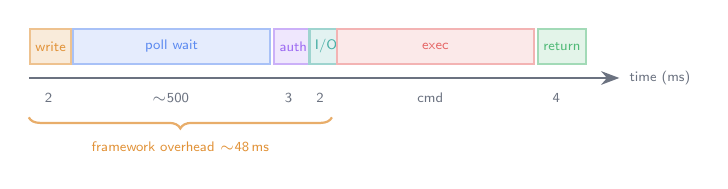
\begin{tikzpicture}[
    >=Stealth,
    phase/.style={draw, thick, minimum height=0.45cm,
                  font=\sffamily\fontsize{5.5}{6.5}\selectfont,
                  inner xsep=2pt, inner ysep=2pt},
    lbl/.style={font=\sffamily\fontsize{5}{6}\selectfont, color=gray1},
]
% Timeline axis
\draw[->, thick, gray1] (0,0) -- (7.5,0)
    node[right, lbl] {time (ms)};

% Phase bars (stacked horizontally)
\node[phase, fill=orange1!15, draw=orange1!45, text=orange1!80,
      minimum width=0.5cm, anchor=west] (w) at (0,0.4) {write};
\node[phase, fill=blue1!12, draw=blue1!40, text=blue1!75,
      minimum width=2.5cm, anchor=west] (poll) at (0.55,0.4) {poll wait};
\node[phase, fill=purple1!12, draw=purple1!40, text=purple1!75,
      minimum width=0.4cm, anchor=west] (hmac) at (3.1,0.4) {auth};
\node[phase, fill=teal1!12, draw=teal1!40, text=teal1!75,
      minimum width=0.3cm, anchor=west] (io) at (3.55,0.4) {I/O};
\node[phase, fill=red1!10, draw=red1!35, text=red1!70,
      minimum width=2.5cm, anchor=west] (exec) at (3.9,0.4) {exec};
\node[phase, fill=green1!12, draw=green1!40, text=green1!75,
      minimum width=0.5cm, anchor=west] (ret) at (6.45,0.4) {return};

% Time labels
\node[lbl] at (0.25,-0.25) {2};
\node[lbl] at (1.8,-0.25) {$\sim$500};
\node[lbl] at (3.3,-0.25) {3};
\node[lbl] at (3.7,-0.25) {2};
\node[lbl] at (5.1,-0.25) {cmd};
\node[lbl] at (6.7,-0.25) {4};

% Brace for overhead
\draw[decorate, decoration={brace, amplitude=4pt, mirror},
      thick, orange1!60] (0,-0.5) -- (3.85,-0.5)
    node[midway, below=5pt, font=\sffamily\fontsize{5.5}{6.5}\selectfont,
         color=orange1!80] {framework overhead $\sim$48\,ms};
\end{tikzpicture}
\caption{\textbf{Latency breakdown.} The poll wait ($\sim$500\,ms average)
dominates discovery time. HMAC verification and file I/O add $\sim$5\,ms.
Command execution time varies by workload.}
\label{fig:latency}
\end{figure}

\subsection{Comparison with Alternatives}

\begin{table}[h]
\centering
\caption{Comparison with alternative dom0 access mechanisms.}
\label{tab:comparison}
\small
\begin{tabular}{@{}lcccc@{}}
\toprule
\textbf{Property} & \textbf{Manual} & \textbf{Qrexec} &
    \textbf{SSH$^\dagger$} & \textbf{Proposed} \\
\midrule
Ad-hoc commands   & \cmark & \xmark & \cmark & \cmark \\
Authentication    & Physical & Policy & Keys & HMAC-256 \\
Audit trail       & \xmark & Partial & syslog & \cmark \\
Multi-VM          & \cmark & Per-svc & \cmark & \cmark \\
Input validation  & Human & \xmark & \xmark & \cmark \\
Timeout control   & Manual & \xmark & \cmark & \cmark \\
Scriptable        & \xmark & \cmark & \cmark & \cmark \\
Pull model        & N/A & \xmark & \xmark & \cmark \\
No NIC required   & \cmark & \cmark & \xmark & \cmark \\
\bottomrule
\multicolumn{5}{@{}l}{\footnotesize $^\dagger$Hypothetical; dom0
has no NIC, making SSH impossible.}
\end{tabular}
\end{table}

% ─── 8. Applications ─────────────────────────────────────────────
\section{Applications}
\label{sec:applications}

The framework has been validated as the bootstrapping mechanism for
a hypervisor-isolated LLM agent infrastructure that confines
autonomous AI agents within Xen-isolated VMs while providing
airgapped administration from dom0. This application demonstrates
that the file-queue protocol can support complex, long-running
orchestration workflows beyond simple command execution, including
systemd service management, qrexec policy deployment, and vchan
tunnel provisioning---all initiated from an unprivileged VM through
the authenticated queue.

% ─── 9. Related Work ─────────────────────────────────────────────
\section{Related Work}
\label{sec:related}

\textbf{Privilege separation.}
Provos et al.~\cite{provos2003preventing} formalized privilege
separation in OpenSSH. Watson et al.~\cite{watson2010capsicum}
introduced capability-mode sandboxing in Capsicum.
Qubes~OS~\cite{rutkowska2010qubes} extends privilege separation to
the entire desktop. The present work provides a controlled mechanism
for crossing the privilege boundary in this last context.

\textbf{Qubes inter-VM mechanisms.}
Split GPG~\cite{qubes2023splitgpg} isolates cryptographic keys via
qrexec. The U2F proxy~\cite{qubes2024u2f} delegates hardware token
operations. Both require pre-installed handlers; the present
framework generalizes to arbitrary commands.

\textbf{Authenticated RPC systems.}
Kerberos~\cite{neuman2005kerberos} provides network authentication
but requires a network stack and KDC infrastructure.
SPIFFE/SPIRE~\cite{spiffe2024} provides workload identity in
cloud-native environments. The present system's file-based,
network-free authentication is specifically designed for the
constrained dom0 environment.

\textbf{File-based IPC.}
Mailslot and named pipe mechanisms in Windows~\cite{russinovich2012windows}
and Unix domain sockets~\cite{stevens2003unix} provide local IPC.
The present protocol extends file-based IPC across the hypervisor
boundary using the host-initiated qvm-run mechanism as the transport.

\textbf{Agent sandboxing and privilege control (2025).}
IsolateGPT~\cite{wu2025isolategpt} provides execution isolation for
LLM-based agentic systems (NDSS~2025).
Progent~\cite{chen2025progent} introduces programmable privilege
control using a domain-specific policy language.
Cohen et al.~\cite{cohen2025faulttolerant} apply transactional
sandboxing with policy-based interception for AI coding agents,
achieving 100\% interception of high-risk commands. The present
framework enables these agent architectures to cross the dom0
boundary safely.

\textbf{Post-quantum hash-based authentication (2025).}
Recent work on stateless hash-based
signatures~\cite{bernstein2025sphincs} and hybrid hash
frameworks~\cite{nature2025hybridhash} integrating SHA-512 and
BLAKE3 demonstrates that HMAC-based authentication remains a
conservative, quantum-resistant foundation. The present system's
HMAC-SHA256 authentication can be upgraded to post-quantum
constructions as they mature.

\textbf{Container escape vulnerabilities (2025).}
Three critical runc CVEs disclosed in November
2025~\cite{cve2025runc} exploit mount race conditions for full
container breakout, reinforcing the motivation for hypervisor-level
isolation over same-kernel approaches.

% ─── 10. Discussion ──────────────────────────────────────────────
\section{Discussion}
\label{sec:discussion}

\textbf{Limitations.} The framework intentionally weakens the Qubes
security model by enabling VM-to-dom0 command execution. This
trade-off is acknowledged explicitly: the service is transient by
default (L5), requires interactive confirmation to enable, and logs
all activity (L4). The 1-second polling interval introduces latency
unsuitable for real-time control loops.

\textbf{Trust assumptions.} The security model assumes: (a)~the Xen
hypervisor correctly enforces memory isolation, (b)~dom0's filesystem
is not compromised, and (c)~the shared key is not leaked through
side channels. Assumption (a) is shared with all Qubes
applications but has been challenged by recent microarchitectural
attacks (QSB-108,
XSA-471)~\cite{qubes2025qsb108}---demonstrating the need for
ongoing mitigation. Assumptions~(b) and~(c) are mitigated by file
permissions and the out-of-band key exchange.

\textbf{Future work.} Formal verification of the protocol using
TLA+~\cite{lamport2002specifying} or
Tamarin~\cite{meier2013tamarin}; integration with hardware security
modules for key storage; adaptive polling intervals based on
queue activity patterns; migration to post-quantum hash
constructions~\cite{bernstein2025sphincs, nature2025hybridhash}
as standardized alternatives mature; and integration with
privilege-control frameworks~\cite{chen2025progent} to compose
fine-grained application-layer policies with the present
transport-layer authentication.

% ─── 11. Conclusion ──────────────────────────────────────────────
\section{Conclusion}
\label{sec:conclusion}

This paper demonstrates that the tension between strict privilege
separation and practical system administration can be resolved
through a carefully designed pull-model RPC protocol. By preserving
the invariant that the control domain initiates all I/O, using
HMAC-SHA256 for per-command authentication with formal security
guarantees, and implementing five independent defense layers, the
framework provides SSH-like convenience while maintaining
auditability and cryptographic accountability. The minimal
implementation ($\sim$1{,}800 SLOC, zero dependencies) is
deployable in the most constrained environments and has been
validated as a foundation for hypervisor-isolated AI agent
infrastructure.

% ─── References ───────────────────────────────────────────────────
\begin{thebibliography}{35}
\small

\bibitem{rutkowska2010qubes}
J.~Rutkowska and R.~Wojtczuk,
``Qubes OS architecture,''
\textit{Invisible Things Lab}, 2010.

\bibitem{barham2003xen}
P.~Barham et al.,
``Xen and the art of virtualization,''
in \textit{Proc.\ ACM SOSP}, 2003, pp.~164--177.

\bibitem{provos2003preventing}
N.~Provos, M.~Friedl, and P.~Honeyman,
``Preventing privilege escalation,''
in \textit{Proc.\ USENIX Security}, 2003.

\bibitem{watson2010capsicum}
R.~N.~M.~Watson, J.~Anderson, B.~Laurie, and K.~Kennaway,
``Capsicum: Practical capabilities for UNIX,''
in \textit{Proc.\ USENIX Security}, 2010.

\bibitem{saltzer1975protection}
J.~H.~Saltzer and M.~D.~Schroeder,
``The protection of information in computer systems,''
\textit{Proceedings of the IEEE}, vol.~63, no.~9, 1975.

\bibitem{krawczyk1997hmac}
H.~Krawczyk, M.~Bellare, and R.~Canetti,
``HMAC: Keyed-hashing for message authentication,''
\textit{RFC 2104}, IETF, 1997.

\bibitem{bellare2006new}
M.~Bellare,
``New proofs for NMAC and HMAC: Security without collision resistance,''
in \textit{Proc.\ CRYPTO}, 2006.

\bibitem{bellare1996keying}
M.~Bellare, R.~Canetti, and H.~Krawczyk,
``Keying hash functions for message authentication,''
in \textit{Proc.\ CRYPTO}, 1996.

\bibitem{xi2023rise}
Z.~Xi et al.,
``The rise and potential of large language model based agents: A survey,''
\textit{arXiv:2309.07864}, 2023.

\bibitem{openai2024agents}
OpenAI,
``Practices for governing agentic AI systems,''
\textit{OpenAI Research}, 2024.

\bibitem{qubes2024qrexec}
Qubes~OS Project,
``Qrexec: Inter-domain communication,''
\textit{Qubes~OS Documentation}, 2024.

\bibitem{qubes2024vchan}
Qubes~OS Project,
``Vchan: Xen shared memory communication,''
\textit{Qubes~OS Documentation}, 2024.

\bibitem{nist800-53}
NIST,
``Security and privacy controls for information systems and organizations,''
\textit{NIST SP 800-53 Rev.~5}, 2020.

\bibitem{bishop2003computer}
M.~Bishop,
\textit{Computer Security: Art and Science}.
Addison-Wesley, 2003.

\bibitem{nist800-90a}
NIST,
``Recommendation for random number generation using deterministic
random bit generators,''
\textit{NIST SP 800-90A Rev.~1}, 2015.

\bibitem{python2024hmac}
Python Software Foundation,
``hmac --- Keyed-hashing for message authentication,''
\textit{Python Standard Library Documentation}, 2024.

\bibitem{brumley2005remote}
D.~Brumley and D.~Boneh,
``Remote timing attacks are practical,''
\textit{Computer Networks}, vol.~48, no.~5, pp.~701--716, 2005.

\bibitem{bernstein2012security}
D.~J.~Bernstein,
``The security impact of a new cryptographic library,''
in \textit{Proc.\ LATINCRYPT}, 2012.

\bibitem{crosby2003denial}
S.~A.~Crosby and D.~S.~Wallach,
``Denial of service via algorithmic complexity attacks,''
in \textit{Proc.\ USENIX Security}, 2003.

\bibitem{halfond2006classification}
W.~G.~Halfond, J.~Viegas, and A.~Orso,
``A classification of SQL-injection attacks and countermeasures,''
in \textit{Proc.\ IEEE ISSSE}, 2006.

\bibitem{poettering2010systemd}
L.~Poettering,
``systemd: System and session manager,''
\textit{freedesktop.org}, 2010.

\bibitem{oliner2012advances}
A.~Oliner, A.~Ganapathi, and W.~Xu,
``Advances and challenges in log analysis,''
\textit{Communications of the ACM}, vol.~55, no.~2, 2012.

\bibitem{qubes2023splitgpg}
Qubes~OS Project,
``Split GPG,''
\textit{Qubes~OS Documentation}, 2023.

\bibitem{qubes2024u2f}
Qubes~OS Project,
``U2F proxy,''
\textit{Qubes~OS Documentation}, 2024.

\bibitem{qubes2024builder}
Qubes~OS Project,
``Qubes Builder v2,''
\textit{Qubes~OS Documentation}, 2024.

\bibitem{neuman2005kerberos}
C.~Neuman, T.~Yu, S.~Hartman, and K.~Raeburn,
``The Kerberos network authentication service (V5),''
\textit{RFC 4120}, IETF, 2005.

\bibitem{spiffe2024}
Cloud Native Computing Foundation,
``SPIFFE: Secure Production Identity Framework for Everyone,''
\textit{CNCF Specification}, 2024.
\url{https://spiffe.io/}

\bibitem{russinovich2012windows}
M.~E.~Russinovich, D.~A.~Solomon, and A.~Ionescu,
\textit{Windows Internals}, 6th ed.
Microsoft Press, 2012.

\bibitem{stevens2003unix}
W.~R.~Stevens, B.~Fenner, and A.~M.~Rudoff,
\textit{UNIX Network Programming}, 3rd ed.
Addison-Wesley, 2003.

\bibitem{czerwinski2004diary}
M.~Czerwinski, E.~Horvitz, and S.~Wilhite,
``A diary study of task switching and interruptions,''
in \textit{Proc.\ ACM CHI}, 2004.

\bibitem{lamport2002specifying}
L.~Lamport,
\textit{Specifying Systems: The TLA+ Language and Tools for Hardware
and Software Engineers}.
Addison-Wesley, 2002.

\bibitem{meier2013tamarin}
S.~Meier, B.~Schmidt, C.~Cremers, and D.~Basin,
``The TAMARIN prover for the symbolic analysis of security protocols,''
in \textit{Proc.\ CAV}, 2013.

\bibitem{wu2025isolategpt}
S.~Wu, H.~Duan, Y.~Wang, et al.,
``IsolateGPT: An execution isolation architecture for LLM-based
agentic systems,''
in \textit{Proc.\ NDSS}, 2025.

\bibitem{chen2025progent}
S.~Chen, Z.~Wang, S.~Arora, et al.,
``Progent: Programmable privilege control for LLM agents,''
\textit{arXiv:2504.11703}, 2025.

\bibitem{cohen2025faulttolerant}
I.~Cohen, A.~Levy, et al.,
``Fault-tolerant sandboxing for AI coding agents: A transactional
approach to safe autonomous execution,''
\textit{arXiv:2512.12806}, 2025.

\bibitem{bernstein2025sphincs}
D.~Aumasson, D.~Bernstein, et al.,
``Stateless hash-based signatures for post-quantum security keys,''
\textit{IACR ePrint}, 2025/298.

\bibitem{nature2025hybridhash}
A.~Khan, S.~Malik, et al.,
``A hybrid hash framework for post quantum secure zero knowledge
identification,''
\textit{Scientific Reports}, vol.~15, 2025.

\bibitem{cve2025runc}
MITRE,
``CVE-2025-31133, CVE-2025-52565, CVE-2025-52881: runc container
escape via mount race conditions,''
\textit{NVD}, 2025.

\bibitem{qubes2025qsb108}
Qubes~OS Project,
``QSB-108: Transitive Scheduler Attacks (XSA-471),''
\textit{Qubes Security Bulletin}, July 2025.

\bibitem{ieee2025qubes}
B.~Singh, R.~Kumar, et al.,
``Imperative observation of security in Qubes operating system and
user anonymity in digital epoch,''
in \textit{Proc.\ IEEE ICCCSP}, 2025.

\end{thebibliography}

\end{document}
